\chapter{Results}
Chapter 5 reports the performance measurements and compares the three Linux translation implementations against a native Dual-Stack baseline across the three environments introduced in Chapter 4. The goal is to quantify the translation overhead of a CLAT-based path relative to Dual-Stack along two dimensions: TCP throughput and ICMP round-trip time (RTT). Sections 5.1 and 5.2 present the empirical results, Section 5.3 synthesizes and interprets the findings across environments and implementations and Section 5.4 summarizes practical challenges encountered during measurement and their mitigations.

Because the three environments differ in virtualization and CPU topology absolute numbers are not directly comparable across environments. Instead, the within-environment comparison to the IPv6 baseline is the primary focus. 

\section{Throughput}
In this section all figures have the time in seconds on the x-Axis and the throughput in Mbits/s on the y-Axis. The first measurements were conducted in the AWS environment.
\begin{figure}[H]
    \centering
    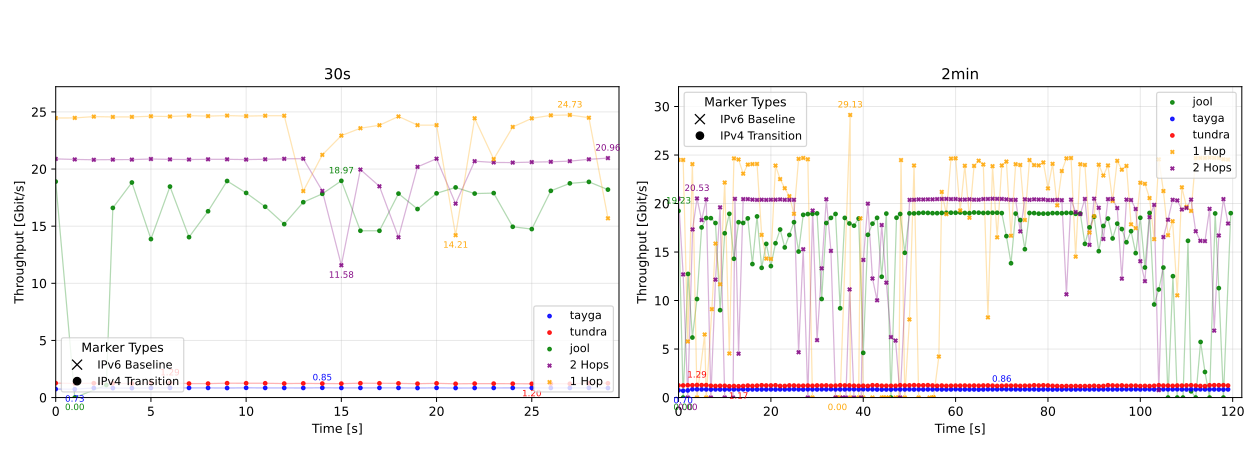
\includegraphics[width=1\textwidth]{resources/plots/CombinedPlot/TCP/AWS_tcp_sameScale_kvm-clock_linear.png}
    \caption{AWS cloud environment, KVM-clock, linear scale}
    \label{fig:AWS_tcp_sameScale_kvm-clock_linear}

\end{figure}
\begin{figure}[H]
    \centering
    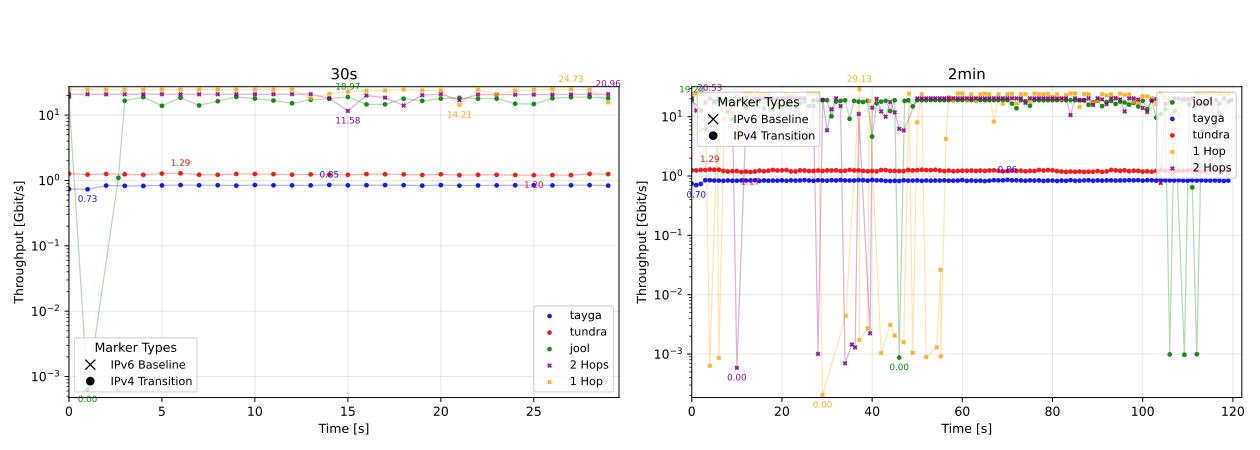
\includegraphics[width=1\textwidth]{resources/plots/CombinedPlot/TCP/AWS_tcp_sameScale_kvm-clock_log.png}
    \caption{AWS cloud environment, kvm-clock, logarithmic scale}
    \label{fig:AWS_tcp_sameScale_kvm-clock_log}

\end{figure}

Figures \ref{fig:AWS_tcp_sameScale_kvm-clock_linear} shows the initial TCP throughput results for the AWS environment in linear and logarithmic y-Axis scaling. Tayga and Tundra show stable, consistent performance across repeated runs. 
In contrast, both the native IPv6 baseline and Jool show large variance and no clear trend, suggesting measurement instability rather than a deterministic effect of the datapath.

Given the constant topology and parameters, this pattern pointed to a timing artifact on the host rather than a translator-specific issue. It was hypothesized that the guest clocksource used by iperf3 and the kernel (kvm-clock) might be introducing jitter under load. To test this, we repeated the measurements after switching the guest clocksource from kvm-clock to hpet. 
The results are presented in the following Figure \ref{fig:AWS_tcp_sameScale_hpet_log}.

\begin{figure}[H]
    \centering
    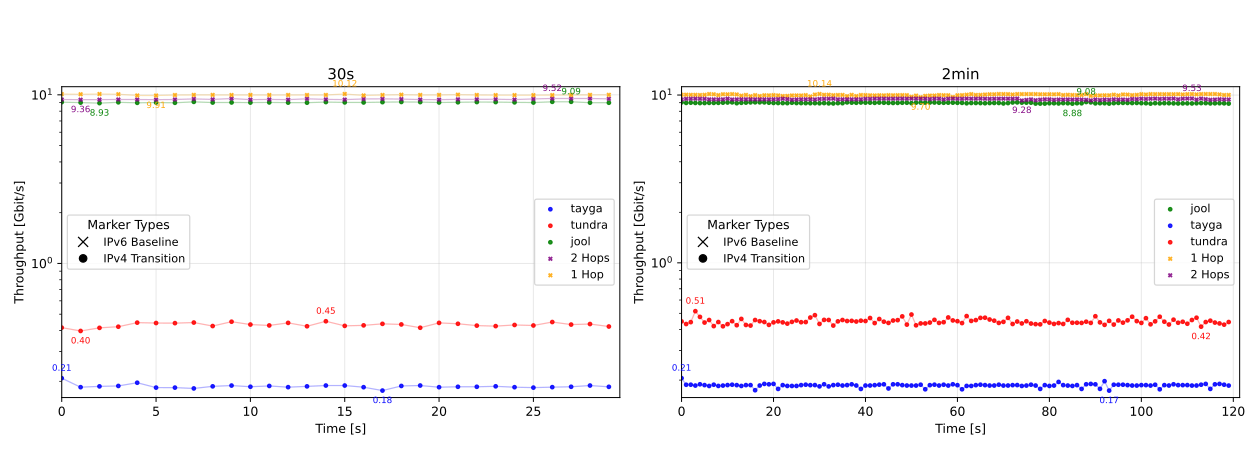
\includegraphics[width=1\textwidth]{resources/plots/CombinedPlot/TCP/AWS_tcp_sameScale_hpet_log.png}
    \caption{AWS cloud environment, hpet, log scale}
    \label{fig:AWS_tcp_sameScale_hpet_log}

\end{figure}

After switching the clocksource to hpet, the single-axis plots still appeared compressed at the extremes: the IPv6 baseline and jool clustered near the top of the axis while the CLAT cases clustered near the bottom. To improve readability, a dual-y-axis figure was introduced: the left y‑axis is scaled for the IPv6 baseline, and the right y‑axis is scaled for the IPv4 translation methods. This separates the ranges and makes differences within each group visible.

\begin{figure}[H]
    \centering
    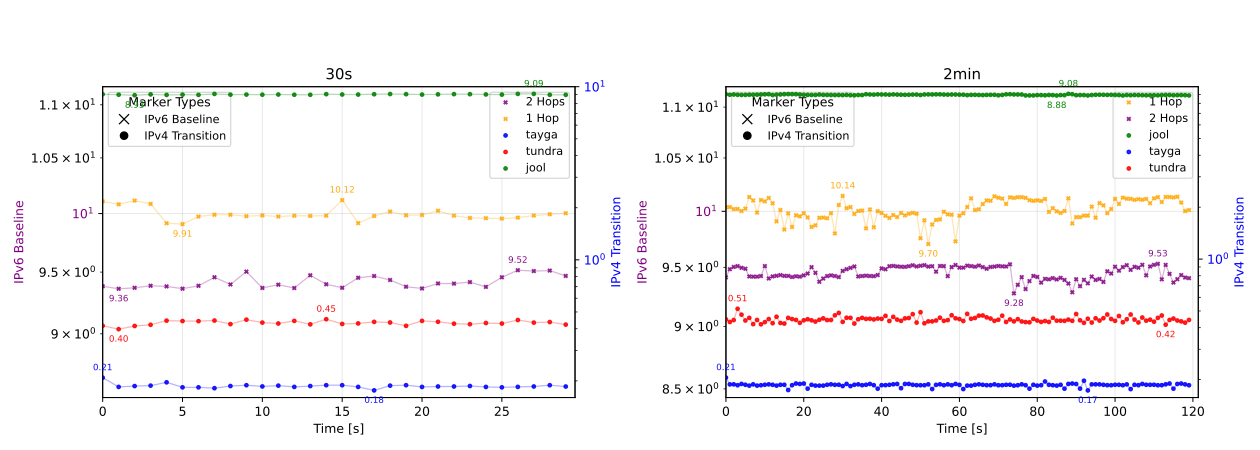
\includegraphics[width=1\textwidth]{resources/plots/JitterPlot/AWS_tcp_dualAxis_hpet_log.png}
    \caption{AWS Throughput Results, hpet, dual-y-axis, log scale}
    \label{fig:AWS_tcp_dualAxis_hpet_log}
\end{figure}

Even with HPET and the dual-y-axis view, the IPv6 baseline shows step‑like jumps rather than a smooth distribution, indicating high amounts of jitter.

Because these irregularities persist despite the clocksource change and improved plotting, the experiments where moved to a local setup to reduce potential platform‑induced artifacts. 
The next figures presents those results.

\paragraph{Local Machine Results}

The following figures show the results from the local machine environment. 
Starting with the results for the single local machine setup. 

\begin{figure}[H]
    \centering
    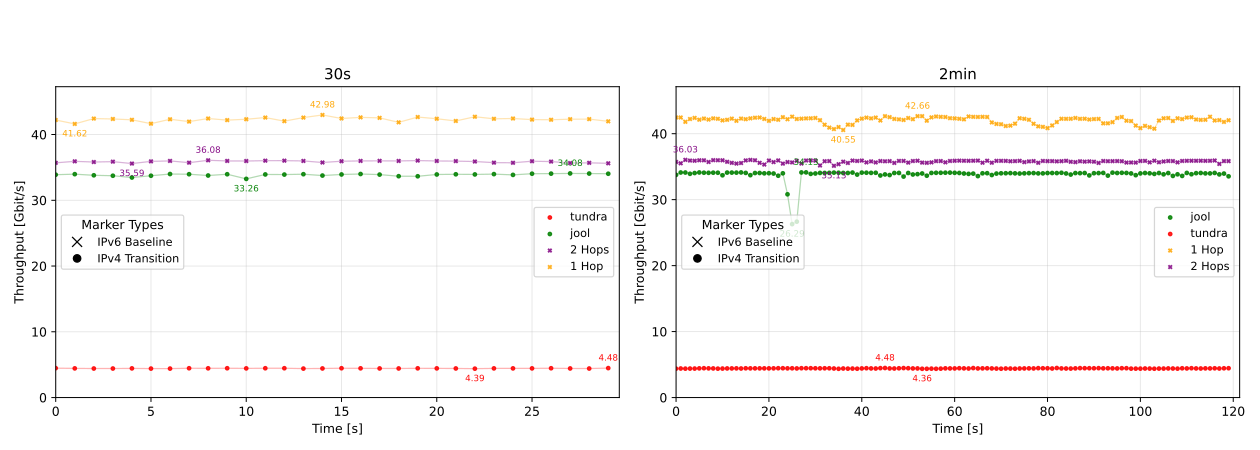
\includegraphics[width=1\textwidth]{resources/plots/CombinedPlot/TCP/Single_tcp_sameScale_tsc_linear.png}
    \caption{Single local machine, tsc, linear scale}
    \label{fig:Local_tcp_sameScale_tsc_linear}
\end{figure}

For consistency we also switched the clocksource to hpet in the local machine environment.

\begin{figure}[H]
    \centering
    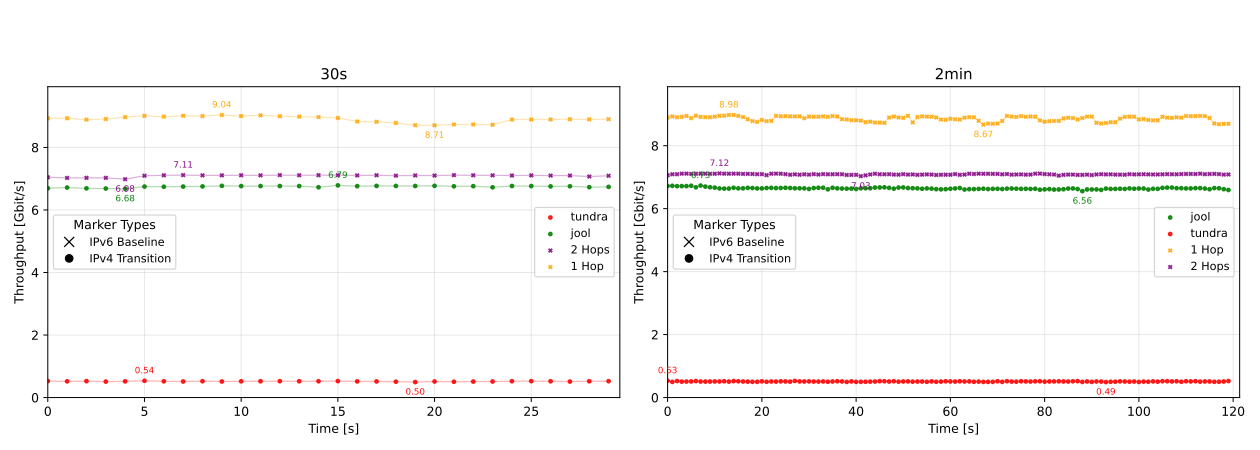
\includegraphics[width=1\textwidth]{resources/plots/CombinedPlot/TCP/Single_tcp_sameScale_hpet_linear.png}
    \caption{Single local machine, hpet, linear scale}
    \label{fig:Local_tcp_sameScale_hpet_linear}
\end{figure}

Switching to the local setup resulted in noticably more stable TCP throughput for both the IPv6 baseline and the CLAT cases. Variability is substantially reduced compared to the AWS runs and repeated measurements cluster tightly around their central values.

Baseline behavior matches expectations: the one-hop IPv6 baseline sustains higher throughput than the two-hop baseline. The observed means are approximately 41.61 Gbit/s for the one-hop path versus 35.84 Gbit/s for the two-hop path, reflecting the additional namespace hop and overhead.

Within the local setup, Jool consistently delivers much higher throughput than Tundra. Under the TSC clocksource (Figure \ref{fig:Local_tcp_sameScale_tsc_linear}), mean throughput is about 33.7 Gbit/s for Jool versus 4.46 Gbit/s for Tundra (roughly 7 times higher). With HPET (Figure \ref{fig:Local_tcp_sameScale_hpet_linear}), the relative ordering is unchanged, with means of about 6.735 Gbit/s for Jool and 0.512 Gbit/s for Tundra (over 10 times higher). Because the absolute levels differ across clocksources, comparisons should be made within each clocksource. The discussion of timing effects and datapath mechanisms is delayed to Section 5.3.
Tayga measurements are absent in this environment. The reasons are detailed in Section 5.3. Given that Tayga and Tundra are both user-space, stateless CLAT implementations with similar behavior, we use Tundra as a representative user-space translator here. The AWS results support this choice, showing comparable performance between the two.
Figure \ref{fig:Local_tcp_dualAxis_hpet_linear} illustrates, in contrast to the earlier AWS dual-y-axis plot, a significantly more stable IPv6 baseline and a clear distinction between the two CLAT implementations. 

\begin{figure}[H]
    \centering
    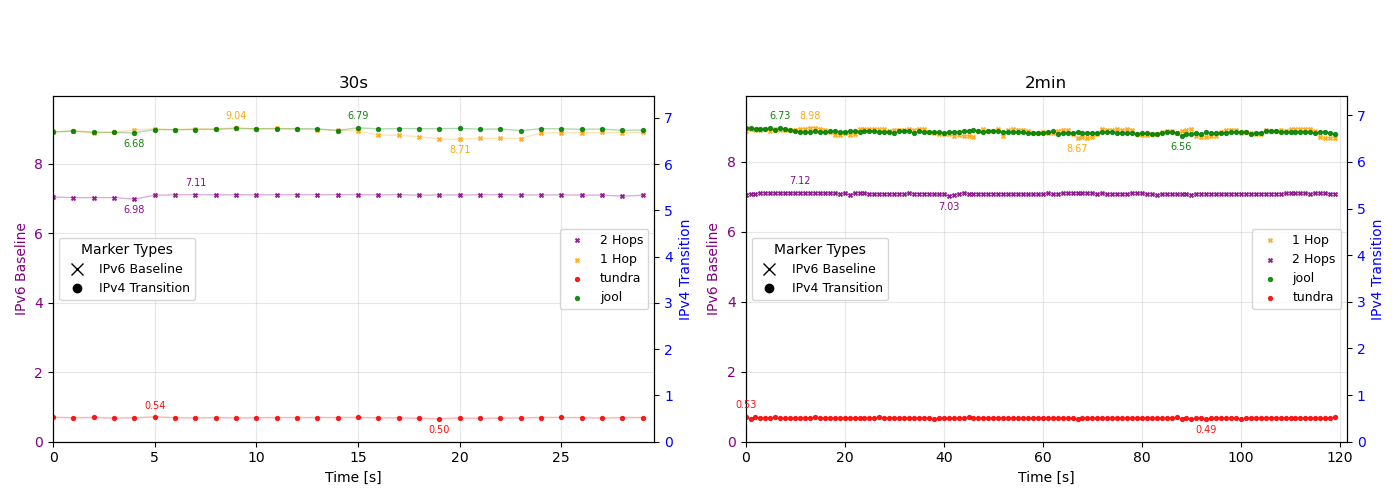
\includegraphics[width=1\textwidth]{resources/plots/JitterPlot/Single_tcp_dualAxis_hpet_linear.png}
    \caption{Single local machine, hpet, dual-y-axis, linear scale}
    \label{fig:Local_tcp_dualAxis_hpet_linear}
\end{figure}

For instance, the range of the IPv6 baseline for two hops has decreased from 0.25 Gbit/s in AWS to about 0.09 Gbit/s in the local setup, indicating a more stable measurement environment.

\paragraph{Dual Machine Local Setup Results}
The final environment for measuring TCP throughput performance is the dual-machine local setup. The following figures show the results for this environment.

\begin{figure}[H]
    \centering
    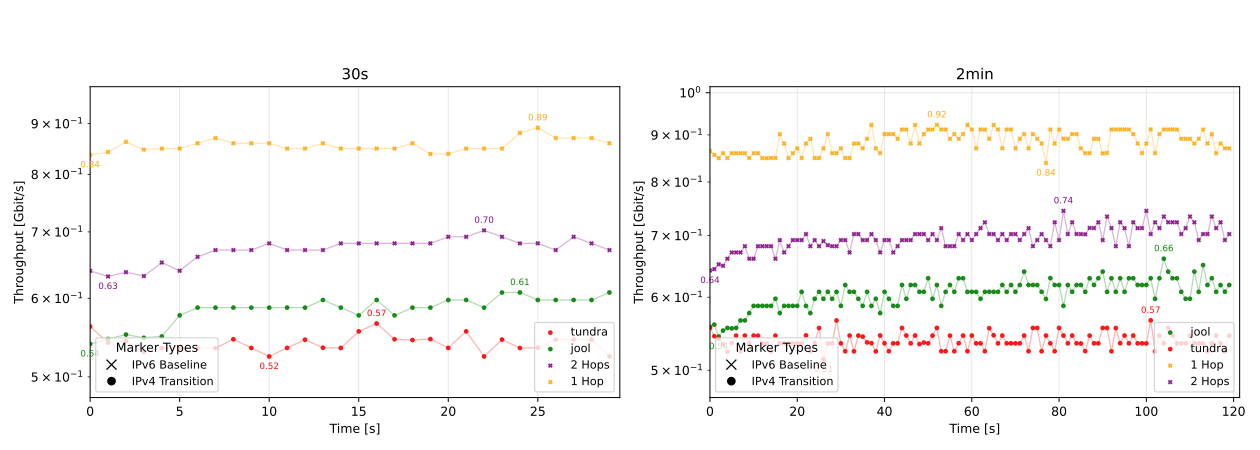
\includegraphics[width=1\textwidth]{resources/plots/CombinedPlot/TCP/Double_tcp_sameScale_hpet_log.png}
    \caption{Dual local machines, hpet, log scale}
    \label{fig:Dual_tcp_sameScale_hpet_log}
\end{figure}

\begin{figure}[H]
    \centering
    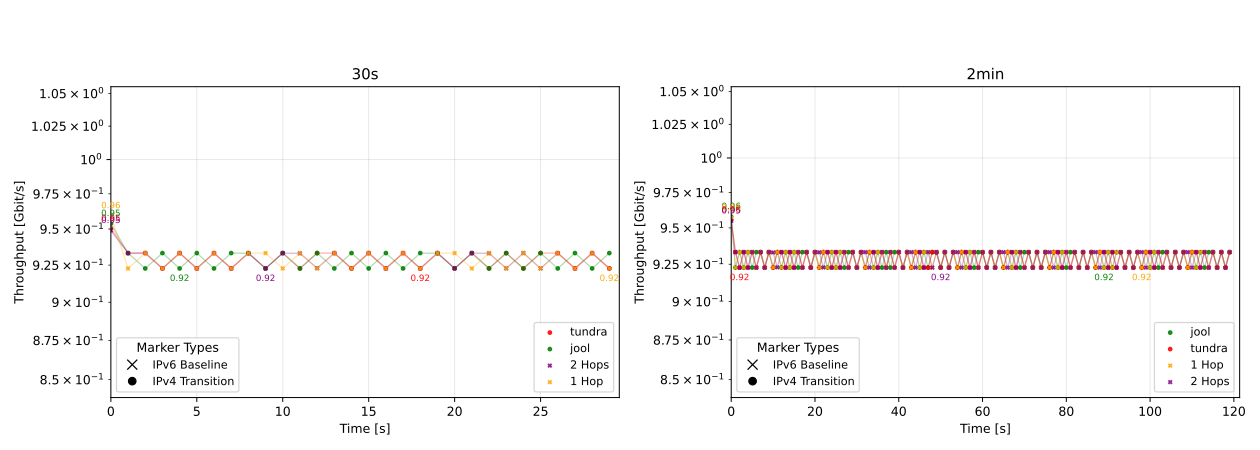
\includegraphics[width=1\textwidth]{resources/plots/CombinedPlot/TCP/Double_tcp_sameScale_tsc_log.png}
    \caption{Dual local machines, tsc, log scale}
    \label{fig:Dual_tcp_sameScale_tsc_log}
\end{figure}

Noticably the throughput values are significantly lower than for the previous environment. Now Jool peakes at 0.66 Gbit/s (Figure \ref{fig:Dual_tcp_sameScale_hpet_log}) and 
Tundra at 0.57 Gbit/s (Figure \ref{fig:Dual_tcp_sameScale_hpet_log}). The big difference between Jool and Tundra has almost disappeared.
This outcome is expected, as the setup relies on Cat5e Ethernet links with a maximum capacity of 1 Gbit/s between machines, creating a bottleneck compared to the loopback interface used in the previous setup.
The maximum achievable throughput is therefore limited by the link speed. This is reflected in Figure \ref{fig:Dual_tcp_sameScale_tsc_log}, where all datapoints are capped at 1 Gbit/s.

We observe here as well that Jool delivers the best performance, consistent with the single-machine setup. 
The slight upward trend is likely attributable to TCP congestion control mechanisms (with cubic being used in the dual-machine setup).
Again, looking at the dual-y-axis plot in Figure \ref{fig:Dual_tcp_dualAxis_hpet_log} for this scenario, 
the IPv6 baseline shows a stable throughput compared to the AWS environment.
\begin{figure}[H]
    \centering
    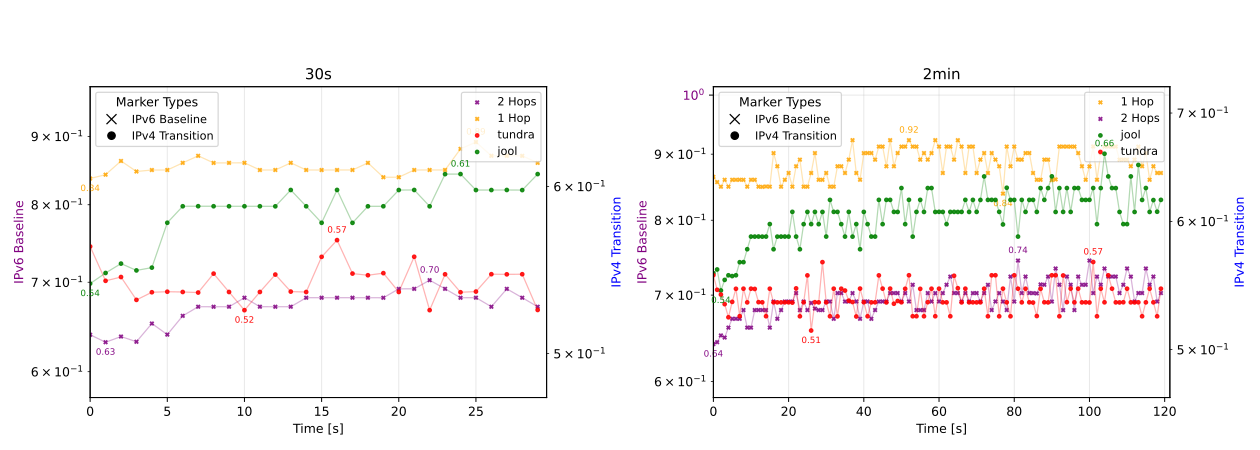
\includegraphics[width=1\textwidth]{resources/plots/JitterPlot/Double_tcp_dualAxis_hpet_log.png}
    \caption{Single local machine, hpet, dual-y-axis, log scale}
    \label{fig:Local_tcp_dualAxis_hpet_log}
\end{figure}


\section{RTT}
The following figures show the RTT measurements for the AWS environment first.

\begin{figure}[H]
    \centering
    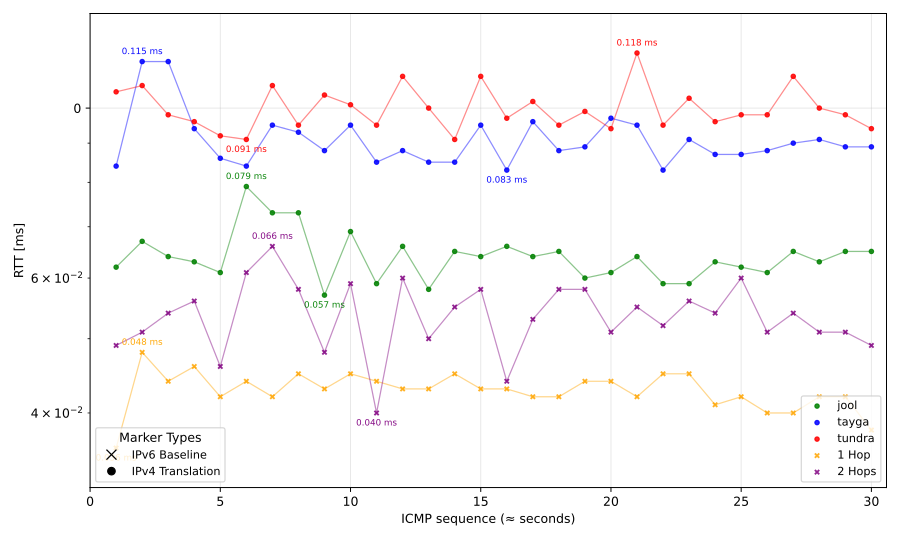
\includegraphics[width=1\textwidth]{resources/plots/CombinedPlot/RTT/AWS_ping_rtt_Ping_30s_log.png}
    \caption{AWS cloud environment, hpet, log scale}
    \label{fig:AWS_icmp_sameScale_hpet_log}

\end{figure}

The results from Figure \ref{fig:AWS_icmp_sameScale_hpet_log} show a clear distinction between the IPv6 baseline and the CLAT implementations. 
This indicates that the translation process introduces additional latency, as expected.
The baseline RTT for one hop is around 0.045 ms and for two hops around 0.052 ms.
Jool again outperforms the user-space implementations, with a mean RTT of around 0.065 ms compared to around 0.086 ms for Tayga and 0.095 ms for Tundra.

The following figures show the results for the single local machine environment.

\begin{figure}[H]
    \centering
    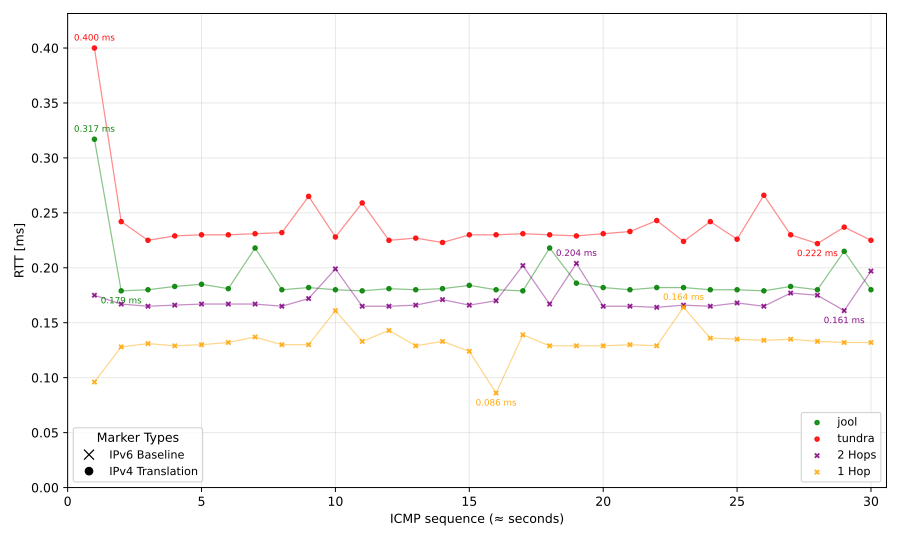
\includegraphics[width=1\textwidth]{resources/plots/CombinedPlot/RTT/Single_ping_rtt_Ping_30s_linear.png}
    \caption{Single local machine environment, hpet, linear scale}
    \label{fig:Local_icmp_sameScale_hpet_linear}
\end{figure}

The results from Figure \ref{fig:Local_icmp_sameScale_hpet_linear} indicate that the single local machine environment exhibits higher RTT values across all implementations compared to the AWS environment.
This is likely due to the weaker hardware of the local machine compared to the AWS instance.
Jool again shows the best performance among the CLAT implementations, with a mean RTT of around 0.182 ms, while Tundra has a RTT mean of around 0.25 ms.

For the dual local machine environment this trend continues.

\begin{figure}[H]
    \centering
    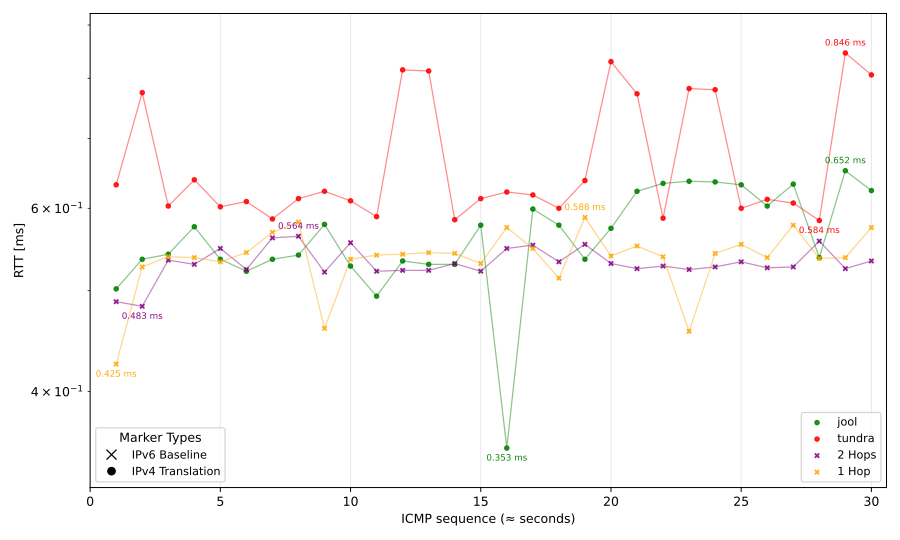
\includegraphics[width=1\textwidth]{resources/plots/CombinedPlot/RTT/Double_ping_rtt_Ping_30s_log.png}
    \caption{Dual local machines environment, hpet, log scale}
    \label{fig:Dual_icmp_sameScale_hpet_log}
\end{figure}

Figure \ref{fig:Dual_icmp_sameScale_hpet_log} shows that the dual local machine environment has the highest RTT values among all environments.
The reason for this is the additional network hop between the two machines, which introduces extra latency.
The additional hop between the two machines also adds more variability to the measurements, as seen in the wider spread of RTT values for all implementations.
Nevertheless Jool continues to deliver the best performance among the CLAT implementations. 


\section{Discussion}

\section{Challenges and Solutions}